% !TeX root = document.tex
% !TeX encoding = UTF-8 Unicode

\section{Zero-Dynamics Attack}%
\label{sec:zda}

\subsection{Introduction}%
\label{subsec:ts-introduction}

\begin{slide}{Zero-Dynamics Attack}
  \begin{columns}[c]
    \begin{column}{0.48\textwidth}
      The attacker changes the control signal in a specific direction, taking
      advantage of the system's transmission zeros to change the system's states
      without affecting the system's output.
      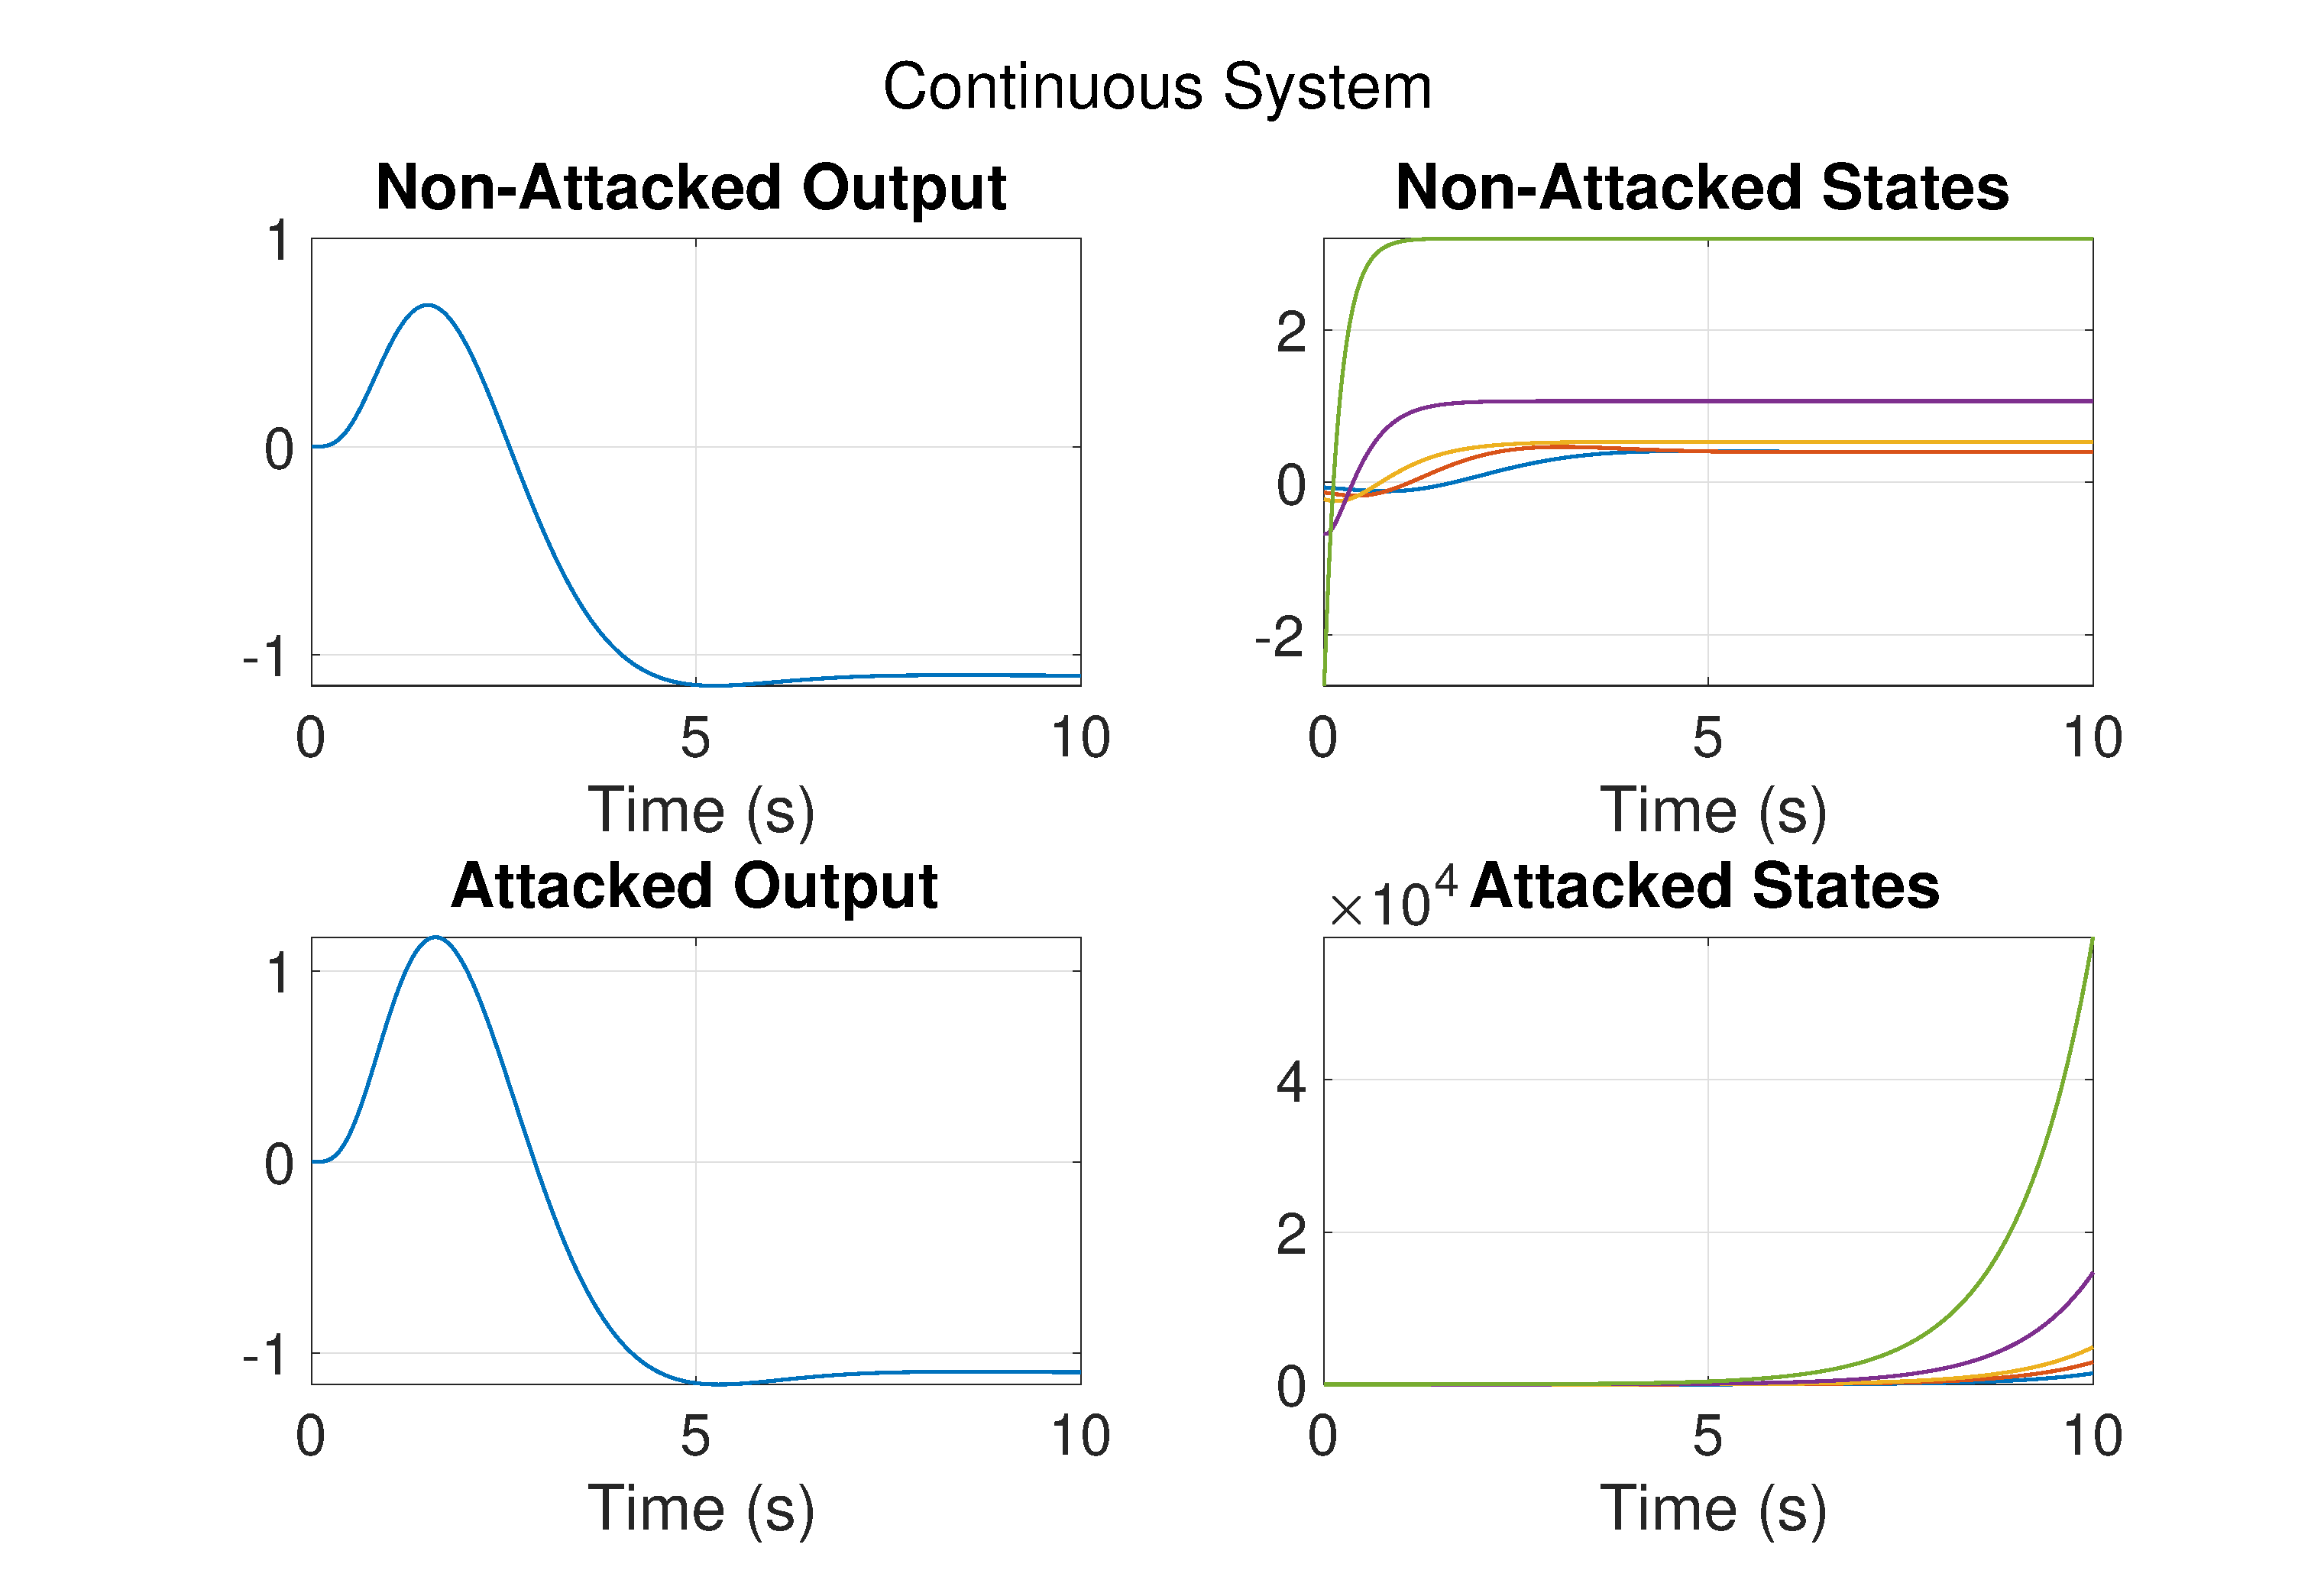
\includegraphics[width=\linewidth]{ct-system}
    \end{column}%
    \hfill%
    \begin{column}{0.48\textwidth}
      \begin{align}
        \dot{x}       & = Ax + Bu                                       \\
        y             & = Cx + Du                                       \\
        \nonumber                                                       \\
        P(s)          & = \begin{bmatrix}
                            sI-A & -B \\
                            C    & D
                          \end{bmatrix},                                \\
        P(s_{0})z_{0} & = 0.                                            \\
        z_{0}         & = \begin{bmatrix} x_{0} \\ a_{0} \end{bmatrix}, \\
        a(t)          & = a_{0}e^{s_{0}t},                              \\
        \tilde{u}(t)  & =u(t) + a(t).
      \end{align}
    \end{column}%
  \end{columns}
\end{slide}

\subsection{Bibliography Review}%
\label{subsec:literature}

\begin{slide}{Current Literature Solutions}
  \begin{columns}[c]
    \begin{column}{0.48\textwidth}
      Current detection schemes in the literature:\\~\\
      \begin{itemize}
        \item Generalized Zero-Order Holders \\
              \textcolor{gray}{\textcite{kim.ryu.ea:zero-dynamics,shim.back.ea:zero-dynamics}}
        \item Modified system models \\
              \textcolor{gray}{\textcite{baniamerian.khorasani.ea:monitoring}}
        \item Topology change \\
              \textcolor{gray}{\textcite{mao.jafarnejadsani.ea:novel}}
      \end{itemize}
    \end{column}%
    \hfill%
    \begin{column}{0.48\textwidth}
      \begin{figure}[ht!]
        \centering
        \resizebox{0.6\linewidth}{!}{%
          \begin{tikzpicture}[node distance=1cm,block/.style={align=center,draw,shape=rectangle,very thick,minimum height=2em, minimum width=3em},>=stealth]
            \node (C) [block]                             {Controller};
            \node (G) [block,above=1.5cm of C]            {System};
            \node (H) [block,below=of C]                  {Time-Scale Observer};
            \node (u) [above left=0.5cm and 1cm of C]     {\(u(t)\)};
            \node (y) [above right=0.5cm and 1cm of C]    {\(y(t)\)};
            \node     [draw,rectangle,dashed,fit=(u) (y)] {Network};

            \draw [->,thick] (C) -| (u) |- (G);
            \draw [->,thick] (G) -| (y) |- (C);
            \draw [->,thick] (u) |- (H);
            \draw [->,thick] (y) |- (H);
          \end{tikzpicture}%
        }
        \caption{Conventional Observer's block diagram}%
      \end{figure}    \end{column}%
  \end{columns}
\end{slide}

\begin{slide}{Current Literature Solutions}
  \begin{columns}[c]
    \begin{column}{0.48\textwidth}
      Current detection schemes in the literature:\\~\\
      \begin{itemize}
        \item Generalized Zero-Order Holders \\
              \textcolor{gray}{\textcite{kim.ryu.ea:zero-dynamics,shim.back.ea:zero-dynamics}}
        \item Modified system models \\
              \textcolor{gray}{\textcite{baniamerian.khorasani.ea:monitoring}}
        \item Topology change \\
              \textcolor{gray}{\textcite{mao.jafarnejadsani.ea:novel}}
      \end{itemize}
    \end{column}%
    \hfill%
    \begin{column}{0.48\textwidth}
      \begin{figure}[ht!]
        \centering
        \resizebox{0.6\linewidth}{!}{%
          \begin{tikzpicture}[node distance=1cm,block/.style={align=center,draw,shape=rectangle,very thick,minimum height=2em, minimum width=3em},>=stealth]
            \node (C) [block]                             {Controller};
            \node (G) [block,above=1.5cm of C]            {System};
            \node (H) [block,above=of G]                  {Time-Scale Observer};
            \node (u) [above left=0.5cm and 1cm of C]     {\(u(t)\)};
            \node (y) [above right=0.5cm and 1cm of C]    {\(y(t)\)};
            \node     [draw,rectangle,dashed,fit=(u) (y)] {Network};

            \draw [->,thick] (C) -| (u) |- (G);
            \draw [->,thick] (G) -| (y) |- (C);
            \draw [->,thick] (u) |- (H);
            \draw [->,thick] (y) |- (H);
          \end{tikzpicture}%
        }
        \caption{Proposed Observer's block diagram}%
      \end{figure}
    \end{column}%
  \end{columns}
\end{slide}
